\documentclass[runningheads]{llncs}

\usepackage[T1]{fontenc}
\usepackage{amssymb}
\usepackage{booktabs}
\usepackage{tikz}
\usetikzlibrary{arrows.meta,positioning}
\usepackage{xcolor}
\usepackage{listings}
\lstset{basicstyle=\ttfamily\scriptsize,breaklines=true,frame=single,columns=fullflexible,
  keywordstyle=\bfseries,commentstyle=\itshape\color{gray},stringstyle=\color{teal!70!black},
  showstringspaces=false}
\usepackage[hidelinks]{hyperref}  % hidelinks: no coloured boxes around links and citations
\usepackage{url}

\begin{document}

\title{SupplyShield: Detecting Malicious Behaviour in Open-Source Packages Before Installation}
\titlerunning{SupplyShield}

\author{Pahuldeep Singh Sodhi}
\authorrunning{Pahuldeep}
\institute{Thapar Institute of Engineering and Technology (TIET), Patiala, India\\
Roll No.: 102306051 \quad Course: Cybersecurity For Mobility Systems\\  \quad Instructor: Dr.\ Rohit Ahuja}

\maketitle

\begin{abstract}
Modern applications are built from hundreds of open-source packages from registries such as PyPI and npm, and attackers exploit this by publishing malicious packages or poisoning updates of popular ones. The free tools most developers use, such as \texttt{pip-audit} and \texttt{npm audit}, only match dependencies against databases of \emph{known} vulnerabilities, so they report a brand-new malicious package as clean. This article presents \emph{SupplyShield}, a dependency-free static analyser for PyPI and npm packages that inspects what a package's code does before installation. It adds \emph{version-diff analysis}, which isolates behaviour introduced by an update, and \emph{attack-chain scoring}, whose weights are \emph{learned} from labelled real and synthetic packages. An optional advisory lookup also reports known vulnerabilities and known malware. The tool was developed in three rounds: synthetic samples, a first real-data run that exposed false alarms, and a final test on real attacks it had never seen. On 20 real hijacked releases of genuine packages, SupplyShield caught 11, against 5 for the specialised tool GuardDog and none for \texttt{pip-audit} and \texttt{npm audit}. Its version diff flagged 11 of 20 real poisoned updates with no false alarms on 20 normal updates, about 100 times faster than GuardDog.

\keywords{Software supply chain security \and Malicious packages \and Static analysis \and PyPI \and npm}
\end{abstract}

%=====================================================================
\section{Introduction}
%=====================================================================

Almost all software people use daily is built on open-source packages. One \texttt{pip install} or \texttt{npm install} can pull in dozens of packages written by strangers, and installation may run their code immediately with the developer's full permissions. Compromising one popular package can therefore reach thousands of projects at once.

Real incidents show the damage. In 2018 a new maintainer of the npm package \texttt{event-stream} added a dependency that stole Bitcoin wallet keys. In 2021 the hijacked \texttt{ua-parser-js} package installed a cryptocurrency miner and stole credentials. In 2024 a backdoor was found in XZ Utils, a compression library present in most Linux systems, planted by a contributor who had spent years earning trust (CVE-2024-3094, CVSS 10)~\cite{nvd_xz}. All three arrived as updates to packages users already trusted.

The free tools most developers use (\texttt{pip-audit}, \texttt{npm audit}, GitHub Dependabot) ask whether a version is \emph{listed in a vulnerability database}. A new malicious package or freshly poisoned update is not listed yet, and that window is exactly when attacks succeed.

In this work, Pahuldeep Singh Sodhi (i) reviews supply chain attacks and detection research; (ii) presents \emph{SupplyShield}, an open-source analyser that never executes the code it inspects, needs no third-party dependencies and explains every finding; (iii) introduces version-diff analysis and attack-chain scoring, and integrates the known-vulnerability check of \texttt{pip-audit} and \texttt{npm audit}; and (iv) evaluates it against \texttt{pip-audit}, \texttt{npm audit}, Bandit and GuardDog. Code, test corpus and scripts are on GitHub.\footnote{\url{https://github.com/PahuldeepSinghSodhi/supplyshield}}

%=====================================================================
\section{Literature Review}\label{sec:lit}
%=====================================================================

\paragraph{Attacks.} Ohm et al.\ analysed 174 malicious packages from real attacks on npm, PyPI and RubyGems (2015--2019)~\cite{ohm2020backstabber}. Attackers either publish a new package, often imitating a popular name (\emph{typosquatting}), or subvert an existing one through a hijacked maintainer account or a malicious dependency. Many packages execute during \emph{installation}, via \texttt{setup.py} or npm \texttt{postinstall} scripts, and most aim to steal credentials, open backdoors or drop further malware. Ladisa et al.\ generalised this into a taxonomy of attacks across the whole supply chain, validated with 17 experts and 134 developers~\cite{ladisa2023taxonomy}.

\paragraph{Detection research.} Duan et al.'s MalOSS combined metadata, static and dynamic analysis, and registry maintainers confirmed 278 of the 339 packages it reported as malicious~\cite{duan2021measuring}. Sejfia and Sch\"afer's Amalfi combines machine-learning classifiers with reproducibility checks and clone detection, and found 95 unknown malicious npm packages in one week~\cite{sejfia2022amalfi}. Both need sandboxes, trained models or registry-scale data, so they are not tools a developer runs before typing \texttt{install}.

\paragraph{Existing tools.} Table~\ref{tab:tools} compares tools developers can use today. Advisory scanners check name and version against vulnerability databases. Bandit flags risky Python constructs such as \texttt{exec}, but knows nothing of installation time, package names or versions. GuardDog, by Datadog, is the closest tool: it applies Semgrep rules to package code and heuristics to registry metadata, and can compare a PyPI release with its GitHub source~\cite{guarddog}. Commercial services such as Socket.dev also analyse behaviour.

\begin{table}[t]
\centering
\caption{Tools available to developers, from their documentation. \checkmark{} = yes, -- = no, $\sim$ = partly, ? = not verified (closed source).}
\label{tab:tools}
\setlength{\tabcolsep}{3pt}
\small
\begin{tabular}{lccccc}
\toprule
 & pip-audit/ & Bandit & GuardDog & Socket & \textbf{Supply-} \\
 & npm audit & & & (paid) & \textbf{Shield} \\
\midrule
Finds new, unlisted malware        & --         & $\sim$     & \checkmark & \checkmark & \checkmark \\
Finds known vulnerable versions     & \checkmark & --         & --         & \checkmark & \checkmark$^{b}$ \\
Install-time context               & --         & --         & \checkmark & \checkmark & \checkmark \\
Typosquatting                      & --         & --         & \checkmark & \checkmark & \checkmark \\
Diff against previous release       & --         & --         & --$^{a}$   & ?          & \checkmark \\
Graded attack-chain scoring        & --         & --         & --         & ?          & \checkmark \\
No third-party dependencies        & --         & --         & --         & n/a        & \checkmark \\
\bottomrule
\multicolumn{6}{l}{\scriptsize $^{a}$ GuardDog compares a release with its source repository, not with the previous release.}\\
\multicolumn{6}{l}{\scriptsize $^{b}$ Optional online lookup (\texttt{-{}-vulns}); all other analysis is offline.}
\end{tabular}
\end{table}

\paragraph{Research gap.} Install-time execution, credential theft and poisoned updates dominate real attacks~\cite{ohm2020backstabber,ladisa2023taxonomy}, yet common free tools cannot see new malicious code, and the strongest detectors need research infrastructure. We found no lightweight open-source tool that judges an update by the behaviour it \emph{adds}, or that scores dangerous \emph{combinations} of signals. SupplyShield targets this gap.

%=====================================================================
\section{Technology Used and Proposed Solution}\label{sec:tech}
%=====================================================================

\paragraph{Threat model.} We assume an attacker who can publish a package to PyPI or npm, either under a new (possibly look-alike) name or as a new release of an existing package after taking over a maintainer account. The attacker's goal is to run code on the developer's or build server's machine, usually at install time, to steal secrets or download further malware. The defender is a developer or a build pipeline that can inspect a package archive before installing it, but does not have a sandbox, a trained model or registry-wide data. SupplyShield is designed for this defender.

\paragraph{Implementation.} SupplyShield is about 1{,}200 lines of Python using only the standard library (\texttt{ast}, \texttt{re}, \texttt{tarfile}, \texttt{zipfile}, \texttt{tomllib}, \texttt{urllib}). It never installs, imports or runs analysed code, works offline except for the optional advisory lookup, and comes with a command-line interface, JSON output, a pre-install guard, 55 unit tests and continuous integration. Fig.~\ref{fig:arch} shows its pipeline.

\begin{figure}[t]
\centering
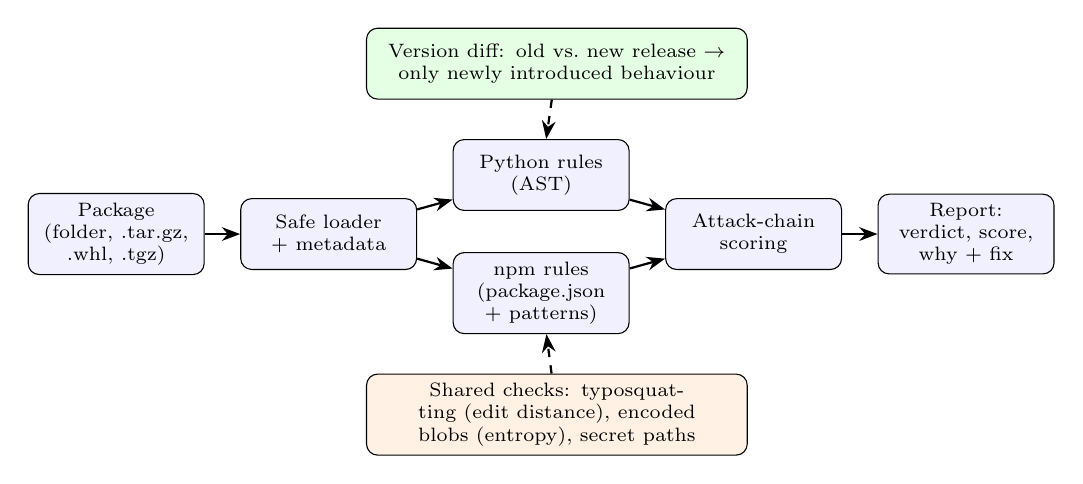
\begin{tikzpicture}[
  box/.style={draw, rounded corners, align=center, font=\scriptsize, minimum height=0.9cm, text width=2.0cm, fill=blue!6},
  arr/.style={-{Stealth}, thick}]
\node[box] (in) {Package\\(folder, .tar.gz,\\.whl, .tgz)};
\node[box, right=0.45cm of in] (load) {Safe loader\\+ metadata};
\node[box, right=0.45cm of load, yshift=0.75cm] (py) {Python rules\\(AST)};
\node[box, right=0.45cm of load, yshift=-0.75cm] (js) {npm rules\\(package.json\\+ patterns)};
\node[box, right=0.45cm of py, yshift=-0.75cm] (score) {Attack-chain\\scoring};
\node[box, right=0.45cm of score] (out) {Report:\\verdict, score,\\why + fix};
\node[box, below=0.5cm of js, text width=4.6cm, xshift=0.2cm, fill=orange!10] (common) {Shared checks: typosquatting (edit distance), encoded blobs (entropy), secret paths};
\node[box, above=0.5cm of py, text width=4.6cm, xshift=0.2cm, fill=green!10] (diff) {Version diff: old vs.\ new release $\rightarrow$ only newly introduced behaviour};
\draw[arr] (in) -- (load);
\draw[arr] (load) -- (py);
\draw[arr] (load) -- (js);
\draw[arr] (py) -- (score);
\draw[arr] (js) -- (score);
\draw[arr] (score) -- (out);
\draw[arr, dashed] (common) -- (js);
\draw[arr, dashed] (diff) -- (py);
\end{tikzpicture}
\caption{SupplyShield architecture.}
\label{fig:arch}
\end{figure}

\paragraph{Loader.} It accepts a folder or archive and extracts archives to a temporary folder, blocking path traversal and symbolic links, then reads the package name, version and dependencies.

\paragraph{Python rules.} Files are parsed into an abstract syntax tree with import aliases resolved, so \texttt{from base64 import b64decode as d; exec(d(...))} is still recognised as a hidden payload. Code in \texttt{setup.py} is marked install-time, and custom install commands are reported. Other rules flag dynamic \texttt{exec}/\texttt{eval}, system commands (critical for download-and-run such as \texttt{curl ... | sh}), network calls, copies of all environment variables, and paths of credential stores such as \texttt{\textasciitilde/.ssh}.

\paragraph{npm rules.} Install scripts are graded as benign native builds (\texttt{node-gyp rebuild}, low), download-and-run commands (critical) or other (medium). Files started by them are marked install-time, and all JavaScript is checked for \texttt{child\_process}, \texttt{eval}, base64 decode-and-execute, network modules, copies of \texttt{process.env}, credential paths and obfuscated identifiers.

\paragraph{Shared checks.} High-entropy strings are flagged as possible hidden payloads. Names are compared with popular packages by Damerau--Levenshtein distance, which counts a swap of neighbouring letters as one edit, so \texttt{lodahs} matches \texttt{lodash}. Credential paths are matched by whole path parts, so a bare \texttt{id\_rsa} counts only next to a real credential folder.

\paragraph{Learned attack-chain scoring.} Single signals are common in legitimate code; malware shows \emph{combinations}, such as install-time code + secret access + network (\emph{data theft}) or obfuscation + execution (\emph{hidden payload}). Instead of hand-picked points, the weight of each signal and chain is learned: a regularised logistic regression on 79 labelled packages (31 malicious, 48 benign), checked with leave-one-out cross-validation, with thresholds chosen on predictions the model had not trained on. It reached AUC 0.90 against 0.87 for hand-set points, and at 90\% detection halved false alarms (21\% to 10\%). Listing~\ref{lst:chains} shows what it learned: look-alike names and hidden code count most, while \texttt{exec} is \emph{more} typical of honest libraries. Scores are shown on a 0--100 scale (60+ \textsc{malicious}, 25--59 \textsc{suspicious}); a critical finding such as download-and-run is always \textsc{malicious}, and the exit code can block a build.

\begin{lstlisting}[language=Python,caption={Learned weights (\texttt{scoring.py}, simplified).},label={lst:chains}]
LEARNED_WEIGHTS = {  # strongest severity per category, 0-3
    "typosquat_level": 1.89, "obfuscation_level": 1.67, "recon_level": 1.54,
    "install_level": 1.38, "secrets_level": 1.13, "network_level": 0.15,
    "process_level": -0.33, "exec_level": -1.14,
    "chain_credential_exfiltration": 1.42, ...}
p = 1 / (1 + exp(-(INTERCEPT + sum(w * x[k] for k, w in LEARNED_WEIGHTS.items()))))
\end{lstlisting}

\paragraph{Version diff.} \texttt{supplyshield diff old new} reports only findings absent from the old release, plus new dependencies, scored on their own; an update that \emph{adds} install-time code is flagged explicitly. This isolates what a poisoned update adds instead of mixing it with behaviour users already accepted (Listing~\ref{lst:out}).

\paragraph{Known vulnerabilities and malware.} With \texttt{-{}-vulns}, SupplyShield also does the job of \texttt{pip-audit} and \texttt{npm audit}: it looks up the exact version in OSV.dev and reports each CVE with its fixed version (on \texttt{requests} 2.19.1 it matched \texttt{pip-audit}'s five vulnerabilities). Known bugs fail the CI exit code but do not raise the malice score; versions listed as confirmed malware are \textsc{malicious}. Only name, ecosystem and version leave the machine.

\begin{lstlisting}[caption={Excerpt of \texttt{supplyshield diff} output for a poisoned update.},label={lst:out}]
Old version 1.0.0: SAFE (0/100)
New version 1.1.0: MALICIOUS (60/100)
Behaviour introduced by update: colorlib 1.0.0 -> 1.1.0 (pypi)
Attack chains detected:
  >> Install-time command execution: runs system commands during installation
CRITICAL PY-DOWNLOAD-EXEC  setup.py:9  [runs at install, NEW in this version]
   code: os.system('curl -s https://collector.example.invalid/stage2.sh | sh')
   why:  A system command downloads something from the internet and runs it
         immediately (e.g. 'curl ... | sh'). This is how second-stage malware is fetched.
   fix:  Do not install. Nothing in a library should download and run remote scripts.
HIGH     PY-INSTALL-HOOK   setup.py:6  [runs at install, NEW in this version]
   code: class Telemetry(setuptools.command.install.install)
\end{lstlisting}

\paragraph{Deployment in developer and agent workflows.} Installs are increasingly typed not only by developers but by build pipelines and AI coding agents, which may pick a package name they have never seen. SupplyShield therefore includes a small pre-install \emph{guard} (\texttt{python -m supplyshield.guard}). It recognises \texttt{pip}, \texttt{uv}, \texttt{npm}, \texttt{yarn} and \texttt{pnpm} install commands, fetches each package without installing it (wheels only for Python, scripts disabled for npm), scans it, and returns exit code 2 to block the command unless every package is \textsc{safe}. The same entry point works in a shell or CI step and as a pre-command hook for an AI coding agent such as Claude Code (Listing~\ref{lst:hook}), where the block reason is returned to the agent so it can choose another package.

\begin{lstlisting}[caption={Placing SupplyShield in front of an AI coding agent's install commands.},label={lst:hook}]
// .claude/settings.json
{"hooks": {"PreToolUse": [{"matcher": "Bash", "hooks": [
    {"type": "command", "command": "python -m supplyshield.guard"}]}]}}

> agent runs: pip install ./samples/pypi/mal-setup-exfil
SupplyShield blocked this install. Choose another package or version, or ask the user.
BLOCKED fastjsonify 0.1.0: MALICIOUS 100/100
        - PY-INSTALL-HOOK: setup.py replaces a standard installation step with custom code...
\end{lstlisting}

%=====================================================================
\section{Evaluation}\label{sec:eval}
%=====================================================================

\paragraph{Method.} Running real malware is unsafe, so we built 20 \emph{inert} packages (10 PyPI, 10 npm) imitating documented attack patterns~\cite{ohm2020backstabber}, with network addresses on the reserved \texttt{.invalid} domain and payloads that only print a message. Each ecosystem has four benign packages (including a harder case: a \texttt{setup.py} that calls \texttt{git}, and a \texttt{node-gyp} add-on) and six malicious ones: install-time credential theft, a base64-hidden payload, environment harvesting, a typosquat, a poisoned update, and one sample written to \emph{evade} SupplyShield. We ran SupplyShield 0.1.0, Bandit 1.9.4 (medium/high issues), \texttt{pip-audit} 2.10.1, \texttt{npm audit} (npm 11.17, scripts disabled) and GuardDog 2.10.0 with Semgrep 1.187, the newest GuardDog that installs on Windows. All tools scanned local folders, where GuardDog skips its registry-metadata rules, including typosquatting.

\begin{table}[t]
\centering
\caption{Detection results (12 malicious, 8 benign packages).}
\label{tab:results}
\setlength{\tabcolsep}{4pt}
\begin{tabular}{lrrrrrrr}
\toprule
Tool & Covered & TP & FN & FP & Precision & Recall & ms/pkg \\
\midrule
\textbf{SupplyShield} & 20 & 10 & 2 & 1 & 0.91 & 0.83 & 6 \\
GuardDog & 20 & 10 & 2 & 1 & 0.91 & 0.83 & 4193 \\
Bandit (medium/high) & 10 & 3 & 3 & 0 & 1.00 & 0.50 & 246 \\
pip-audit & 10 & 0 & 6 & 0 & -- & 0.00 & 585 \\
npm audit & 10 & 0 & 6 & 0 & -- & 0.00 & 1004 \\
\bottomrule
\end{tabular}
\end{table}

\paragraph{Results.} Table~\ref{tab:results} shows the results. \texttt{pip-audit} and \texttt{npm audit} detected nothing: they reported ``no known vulnerabilities'' even for a package that steals the user's npm token, as they are built for known vulnerable versions, not new malware. Bandit caught the three Python packages using \texttt{exec}, \texttt{eval} or network calls, but missed the typosquat and rated \texttt{os.system("curl ... | sh")} in an install hook as \emph{low} severity.

GuardDog matched SupplyShield's totals with different errors: it caught both evasive samples but missed both typosquats, and gives no severity, so a benign \texttt{node-gyp} script and a poisoned \texttt{curl | sh} script looked identical.

\paragraph{Real data, round 2.} We then tested v0.1 on real packages: 20 random \emph{malicious-intent} samples from Datadog's human-triaged dataset~\cite{datadog_dataset} (one excluded: antivirus blocked reading it) and the 40 most-downloaded PyPI and npm packages. Malware was only read, in a temporary folder, then deleted. \texttt{pip-audit} and \texttt{npm audit} again caught nothing, and SupplyShield caught 17 of 19, but it flagged 45\% of popular packages, including \texttt{requests}. Tracing every finding to its file led to general fixes (v0.2): only real connections count as network access, test and documentation files are downgraded, and copying the environment is no longer treated as theft. On 20 unseen popular packages, false alarms fell from 8 to 5.

\paragraph{Real data, round 3: never-seen attacks.} After learning the scoring (v0.3), we ran one final test on data never used for rules or scoring: 20 real \emph{hijacked releases} of genuine packages (Datadog's \emph{compromised} category, e.g.\ \texttt{axios} 1.14.1 and \texttt{eslint-config-prettier}), each with its clean previous release, and 20 further popular packages with their previous releases (Table~\ref{tab:real}). The learned scoring nearly doubled detection, and the version diff caught 11 of 20 poisoned updates with no false alarms on 20 normal updates. Most hijacks \emph{add} an install script that runs packed code or a binary the rules cannot read, a signal the model learned to weight strongly. GuardDog raised fewer false alarms on popular packages but caught less than half as many attacks. v0.3 lost three hijacks that v0.2 had flagged, and \texttt{axios} hid its malware in a newly added dependency, which a per-package scan cannot see.

\begin{table}[t]
\centering
\caption{Never-seen real data: 20 hijacked releases, 20 popular packages, each with its previous release. GuardDog timed out (180\,s) on one benign package.}
\label{tab:real}
\setlength{\tabcolsep}{4pt}
\begin{tabular}{lccc}
\toprule
 & SupplyShield 0.2 & \textbf{SupplyShield 0.3} & GuardDog 2.10 \\
\midrule
Hijacked releases caught & 6/20 & \textbf{11/20} & 5/20 \\
Poisoned updates caught by diff & 2/20 & \textbf{11/20} & -- \\
False alarms, popular packages & 6/20 & 5/20 & 3/19 \\
False alarms, clean pre-attack releases & 5/20 & \textbf{2/20} & -- \\
False alarms, diff on normal updates & 0/20 & \textbf{0/20} & -- \\
Time per package & 0.2\,s & 0.2\,s & 20\,s \\
\bottomrule
\end{tabular}
\end{table}

\paragraph{Discussion.} For packages too new for any advisory database, common free scanners give no protection. Behaviour analysis with learned weights caught over half of real hijacks, more than twice GuardDog's rate, at a hundredth of its cost, and the version diff isolates what an update adds without alarming on normal updates. A quarter of popular packages are still flagged, mostly ones whose real job resembles an attack (\texttt{botocore} reads AWS credentials; \texttt{numpy} runs compilers).

%=====================================================================
\section{Limitations and Conclusion}
%=====================================================================

Samples are small (20 per group, wide intervals), come from one malware dataset that GuardDog itself mostly found, and benign packages are popular ones only. Next steps are scanning newly added dependencies, lowering false alarms on SDK-like packages, larger tests~\cite{ohm2020backstabber}, and pairing static with sandboxed dynamic analysis.

Supply chain attacks turn trust in open-source packages into a route for malware, while common free tools only recognise known problems. SupplyShield shows that a small, dependency-free analyser, refined in three rounds of increasingly real data, can examine what a package does before installation, explain its findings, and reveal what an update adds, catching over half of never-seen real hijacks that \texttt{pip-audit} and \texttt{npm audit} report as clean. Because it is fast and returns a simple exit code, it can sit quietly in front of the install commands of developers, build pipelines and AI coding agents alike.

\bibliographystyle{splncs04}
\bibliography{references}

\end{document}
